\documentclass{report}

\usepackage{url}
\usepackage{graphicx}
\usepackage{makeidx}
\usepackage[adobe-utopia]{mathdesign}

\title{User Manual}

\begin{document}

		\chapter{Graphical Interface}
	
			\emph{Pawned}'s Version 1.1 supports three games: Standard Antichess, 
			Encastle Antichess, and Connect N.
	
			The graphical interface requires that \emph{Java Web Start 
			(JAWS)} is properly installed in your computer.\footnote[1]{\emph{Pawned} 
			does not run on Mac OS X because as of SWT 3.2, SWT applications are 
			not deployable using JAWS on Mac OS X} You may download JAWS from:
				\begin{center}
					\url{http://java.sun.com/products/javawebstart/}				
				\end{center}
			Once installed, you can download \emph{Pawned} from the following website:
				\begin{center}
					\url{http://web.mit.edu/reipince/www/pawned/}				
				\end{center}
			Open or save the pawned.jnlp file in your computer. If you want to be able 
			of loading and saving games, make sure to trust the signature of this 
			application. After loading, you will see \emph{Pawned}'s main window.
				
				%%% Menu and toolbar
				\begin{figure}
					\begin{center}
						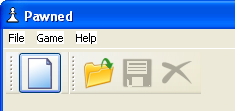
\includegraphics[width=200pt]{img/menu-toolbar.png}
							\caption{Menu and toolbar}
					\end{center}
				\end{figure}
		
				
			On startup, the main window consists of three menu bars, a toolbar, and an 
			empty main panel. After starting a game the main panel will display:
			
				\begin{itemize}
						\item A graphical representation of the board and pieces of the game. 
						\item The names of the players (if they were given) along with the 
									color of the pieces they are using.
						\item A timer for each player that shows how much time left the player 
									has to complete all his moves. If no time limit is selected, 
									an infinite symbol is displayed.
						\item A move history displaying all the moves that have been made 
									througout the game.
				\end{itemize}			
				
			Furthermore, when playing any of the Antichess variants, the main panel 
			will display the pieces each player has captured. A numbering appears
			next to Antichess board, allowing the user to easily reference a cell 
			in it.
				
			\section{Starting a new game}
			
			To start a new game, select File > New Game or click the New Game button in
			the toolbar. This will open a new window (Figure 1.2) where you can choose 
			the settings of the new game. For each one of the players you can:
			
				%%% New Game window antichess
				\begin{figure}
					\begin{center}
						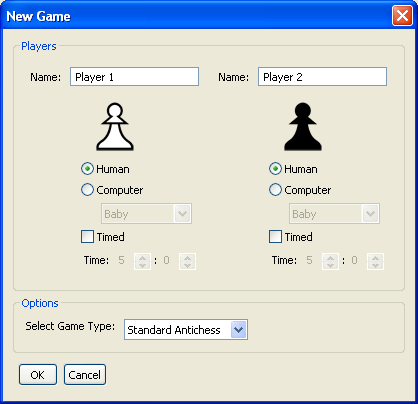
\includegraphics[width=200pt]{img/new-game-1.png}
							\caption{New Game window Standard Antichess options}
					\end{center}
				\end{figure}
				
				%%% New Game window connect 4
				\begin{figure}
					\begin{center}
						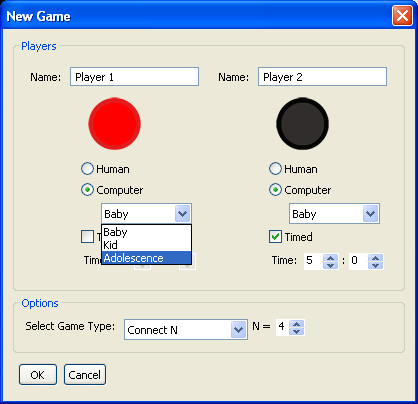
\includegraphics[width=200pt]{img/new-game-2.png}
							\caption{New Game window Connect N options}
					\end{center}
				\end{figure}
				
				\begin{itemize}
					\item Input the name of the player in the 'Name:' text field.
					\item Select between Human or Computer player.
					\item If Computer player is selected, select between three levels of 
								difficulty (Baby, Kid, Adolescence).
					\item Select the Timed checkbox if a timed game is desired. If checked, 
								input the desired time limit in the fields below - minutes in the 
								first field, from 0 to 60, and seconds in the second field, from 0 to
								59 - by either typing the numbers or using the arrows to increment 
								or decrease the time limit displayed as default. \textit{(Note: You
								can not start a game with 0 time in any of the timers)}
				\end{itemize}
			Then, you can select the type of game you want to play. The default is set to
			Standard Antichess, but you can choose to play EnCastle Antichess or Connect N. 
			If you choose to play Connect N, a field to select the value of N will become 
			visible to the right of the Options section. A valid value for n is an integer 
			between 2 and 7 inclusive. The upper bound corresponds to the Connect N's board 
			dimensions that \emph{Pawned} supports (7x6).
			
			Finally, click 'OK' to start the game. At any time you may exit the New Game window
			by clicking 'Cancel'.
			
			If you are playing Antichess, once you click 'OK', the pieces will appear in the 
			board, and the timers, if any, will start to run. No pieces will be displayed for
			Connect N as the board's initial position does not contain any piece. If both 
			players were chosen to be computer players, then the user will be an observer 
			and will not be able of accessing the board in any way. If you are a player, 
			then you will be able of making a move during your turn.
			
			%%% During game
				\begin{figure}
					\begin{center}
						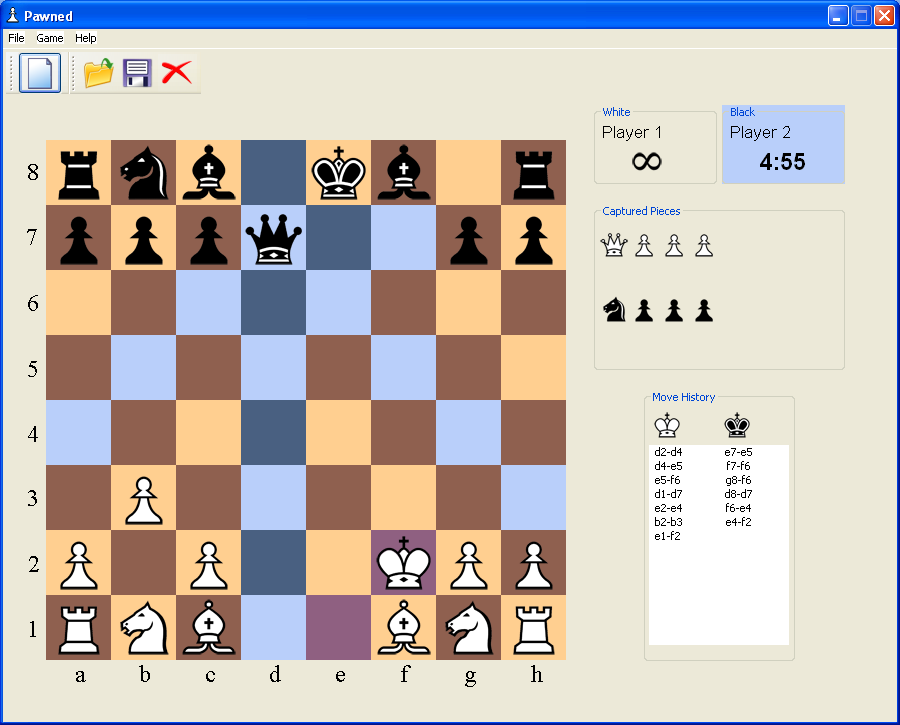
\includegraphics[width=280pt]{img/in-game-1.png}
							\caption{Player 1 is playing with unlimited time, and Player 2 has 4:55 
											minutes left in his timer. It is black player's turn, as is 
											indicated in the players' information display. The possible cells
								      to where Player 2 can move with the Queen are highlighted in blue.
								      The last move made by Player 1 is highlighted in purple.}
					\end{center}
				\end{figure}
			
			You know whose turn it is by looking at the players' information panels at 
			the upper right corner of the main panel: the panel of the player who has
			to play will be highlighted. If you are playing Antichess, the captured 
			pieces are displayed below the players' panels.  At the bottom you can 
			find the move history. The first column corresponds to the move history of 
			the white player and the second column to the history of the black player.
			
			\section{Loading a game}
			
			You can load a game by going to File > Load Game or clicking the Load Game
			button in the toolbar. The Load Game window will be displayed (Figure 1.4).
			
			%%% Load Game
				\begin{figure}
					\begin{center}
						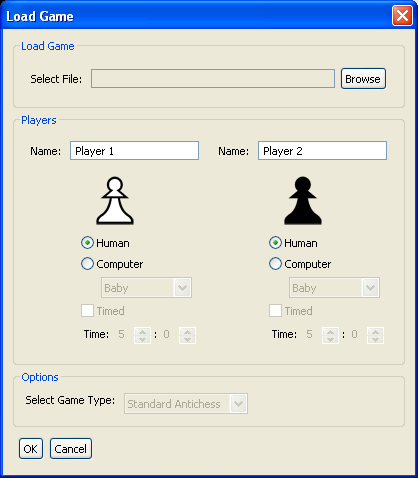
\includegraphics[width=200pt]{img/load-game-1.png}
							\caption{Load Game}						
					\end{center}
				\end{figure}
			
			This window is similar to the New Game window, but it allows you to select a
			file from a File dialog when you click 'Browse' (upper right corner).
			Once you select the Xml game file and click 'Open' in the File dialog,
			the Load Game window will refresh to show the time settings and game type of 
			the saved game (if the game was timed, the time remaining will be displayed
			in the Time fields). You are allowed to change the time settings of the game
			before loading it, and decide the type of players that will play (Human or 
			Computer). However, you will not be able of changing the game type. 
			
			\emph{Pawned} will notify you if the selected game file is invalid or 
			corrupted. Also, it will not let you click 'OK' without selecting a file.
			
			After you are done with the settings, you can click 'OK' to load the game. At 
			any time you may exit the Load Game window by clicking 'Cancel'.
			
			\section{Saving a game}
			
			You can save a game in process by going to File > Save Game or clicking the 
			Save Game button in the toolbar. A File dialog that will let you choose where 
			to save your game will appear. The game will be saved as an Xml file. For
			more information about the format of this file refer to the Appendix. 
			
			%%% Save Game
			\begin{figure}
					\begin{center}
						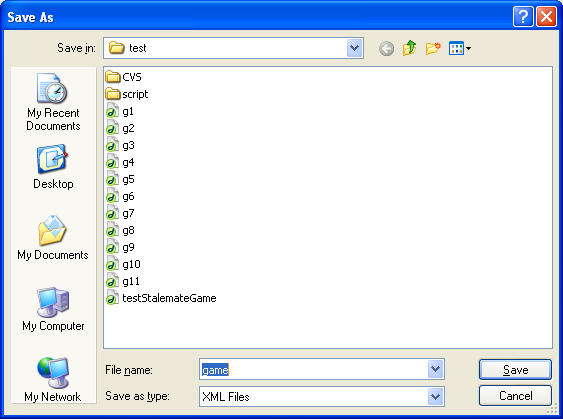
\includegraphics[width=200pt]{img/save-game.png}
							\caption{Save Game}						
					\end{center}
				\end{figure}
			
			\section{Ending a game}
			
			You can choose to end a game in process by going to Game > End Game or clicking
			the End Game button in the toolbar. Ending a game will stop the current game, and
			will leave the display of the game status as it was before ending. 
			\textit{Important: You cannot go back to a game or try to save it after ending it
			using this option.}
			 
			\section{Changing the display options}
			
			Standard Antichess and EnCastle Antichess have three display options set as default:
			
				\begin{itemize}
					\item Highlight Movable Pieces - Highlights the pieces that can be moved
								by the user in a given turn.
					\item Highlight Possible Moves - When the mouse hovers over a movable 
								piece, the cells to where this piece can move are highlighted.
					\item Highlight Last Move - Highlights the last move in the game.
				\end{itemize}
			 
			These settings can be changed by the user at any point during the game by going 
			to Game > Display Options. An option is enabled if there is a checkmark next
			to the text describing it. A click on the option will check or uncheck it. 
			Changes in the display options will be enabled in the next player turn.
			
			\textit{(Note: Connect Four does not support any of these display options)}
			
				%%% Display Options
				\begin{figure}
					\begin{center}
						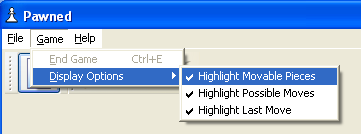
\includegraphics[width=200pt]{img/display-options.png}
							\caption{Display Options}						
					\end{center}
				\end{figure}
			
			\section{Getting help}
			
			The user manual can be accessed by going to Help > User Manual.
			
			\section{Quitting \emph{Pawned}}
			
			You can exit the application by going to File > Quit or by clicking the Close
			button (X) in the upper right corner of the main window.
			
			\section{Hot keys}
			
			Use the following keyboard shortcuts to access some of the basic 
			functionalities of \emph{Pawned}:
			
				\begin{itemize}
					\item New Game - Ctrl + N
					\item Load Game - Ctrl + O
					\item Save Game - Ctrl + S
					\item End Game - Ctrl + E
					\item User Manual - Ctrl + U
					\item Quit - Ctrl + Q
				\end{itemize}			
								
			
			\section{Antichess: Moving the pieces}
			
			In the Antichess games, you can move the pieces by making a first click on
			the piece you want to move, and then making a second click in the cell where
			you want to end. If you make a click on a piece, and later choose not to move
			it, you can	unselect your option by making the second click on the same piece
			or another cell that does not complete a valid move. Any click on a cell that
			does not contain a movable piece will not be counted as a first click.
			
			\section{Connect N: Playing the game}
			
			Making a move in Connect N requires you to click on a hole where your chip can
			be placed. Valid moves are indicated when your mouse hovers over a column
			that is not full. Click the hole and then watch the chip go in! 		
							
				%%% Connect n game
				\begin{figure}
					\begin{center}
						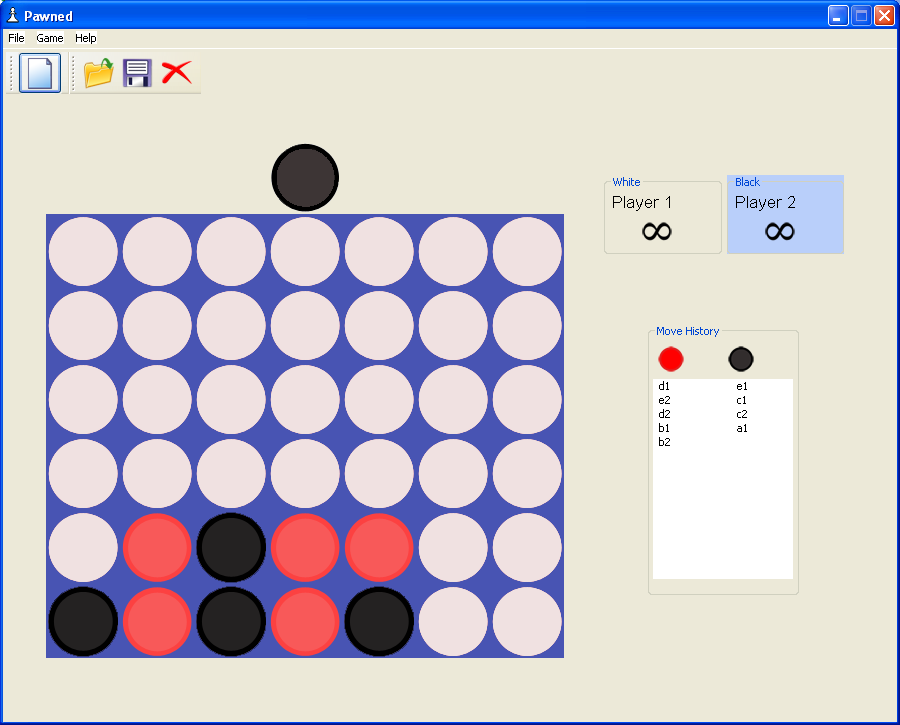
\includegraphics[width=280pt]{img/c4-in-game.png}
							\caption{Playing Connect N}						
					\end{center}
				\end{figure}
			
			
\end{document}
